\documentclass[twoside]{book}

% Packages required by doxygen
\usepackage{fixltx2e}
\usepackage{calc}
\usepackage{doxygen}
\usepackage[export]{adjustbox} % also loads graphicx
\usepackage{graphicx}
\usepackage[utf8]{inputenc}
\usepackage{makeidx}
\usepackage{multicol}
\usepackage{multirow}
\PassOptionsToPackage{warn}{textcomp}
\usepackage{textcomp}
\usepackage[nointegrals]{wasysym}
\usepackage[table]{xcolor}

% Font selection
\usepackage[T1]{fontenc}
\usepackage[scaled=.90]{helvet}
\usepackage{courier}
\usepackage{amssymb}
\usepackage{sectsty}
\renewcommand{\familydefault}{\sfdefault}
\allsectionsfont{%
  \fontseries{bc}\selectfont%
  \color{darkgray}%
}
\renewcommand{\DoxyLabelFont}{%
  \fontseries{bc}\selectfont%
  \color{darkgray}%
}
\newcommand{\+}{\discretionary{\mbox{\scriptsize$\hookleftarrow$}}{}{}}

% Page & text layout
\usepackage{geometry}
\geometry{%
  a4paper,%
  top=2.5cm,%
  bottom=2.5cm,%
  left=2.5cm,%
  right=2.5cm%
}
\tolerance=750
\hfuzz=15pt
\hbadness=750
\setlength{\emergencystretch}{15pt}
\setlength{\parindent}{0cm}
\setlength{\parskip}{0.2cm}
\makeatletter
\renewcommand{\paragraph}{%
  \@startsection{paragraph}{4}{0ex}{-1.0ex}{1.0ex}{%
    \normalfont\normalsize\bfseries\SS@parafont%
  }%
}
\renewcommand{\subparagraph}{%
  \@startsection{subparagraph}{5}{0ex}{-1.0ex}{1.0ex}{%
    \normalfont\normalsize\bfseries\SS@subparafont%
  }%
}
\makeatother

% Headers & footers
\usepackage{fancyhdr}
\pagestyle{fancyplain}
\fancyhead[LE]{\fancyplain{}{\bfseries\thepage}}
\fancyhead[CE]{\fancyplain{}{}}
\fancyhead[RE]{\fancyplain{}{\bfseries\leftmark}}
\fancyhead[LO]{\fancyplain{}{\bfseries\rightmark}}
\fancyhead[CO]{\fancyplain{}{}}
\fancyhead[RO]{\fancyplain{}{\bfseries\thepage}}
\fancyfoot[LE]{\fancyplain{}{}}
\fancyfoot[CE]{\fancyplain{}{}}
\fancyfoot[RE]{\fancyplain{}{\bfseries\scriptsize Generated by Doxygen }}
\fancyfoot[LO]{\fancyplain{}{\bfseries\scriptsize Generated by Doxygen }}
\fancyfoot[CO]{\fancyplain{}{}}
\fancyfoot[RO]{\fancyplain{}{}}
\renewcommand{\footrulewidth}{0.4pt}
\renewcommand{\chaptermark}[1]{%
  \markboth{#1}{}%
}
\renewcommand{\sectionmark}[1]{%
  \markright{\thesection\ #1}%
}

% Indices & bibliography
\usepackage{natbib}
\usepackage[titles]{tocloft}
\setcounter{tocdepth}{3}
\setcounter{secnumdepth}{5}
\makeindex

% Hyperlinks (required, but should be loaded last)
\usepackage{ifpdf}
\ifpdf
  \usepackage[pdftex,pagebackref=true]{hyperref}
\else
  \usepackage[ps2pdf,pagebackref=true]{hyperref}
\fi
\hypersetup{%
  colorlinks=true,%
  linkcolor=blue,%
  citecolor=blue,%
  unicode%
}

% Custom commands
\newcommand{\clearemptydoublepage}{%
  \newpage{\pagestyle{empty}\cleardoublepage}%
}

\usepackage{caption}
\captionsetup{labelsep=space,justification=centering,font={bf},singlelinecheck=off,skip=4pt,position=top}

%===== C O N T E N T S =====

\begin{document}

% Titlepage & ToC
\hypersetup{pageanchor=false,
             bookmarks=true,
             bookmarksnumbered=true,
             pdfencoding=unicode
            }
\pagenumbering{roman}
\begin{titlepage}
\vspace*{7cm}
\begin{center}%
{\Large “assign2prototype” \\[1ex]\large 1 }\\
\vspace*{1cm}
{\large Generated by Doxygen 1.8.11}\\
\end{center}
\end{titlepage}
\clearemptydoublepage
\tableofcontents
\clearemptydoublepage
\pagenumbering{arabic}
\hypersetup{pageanchor=true}

%--- Begin generated contents ---
\chapter{Hierarchical Index}
\section{Class Hierarchy}
This inheritance list is sorted roughly, but not completely, alphabetically\+:\begin{DoxyCompactList}
\item \contentsline{section}{Factory}{\pageref{class_factory}}{}
\item \contentsline{section}{Member}{\pageref{class_member}}{}
\begin{DoxyCompactList}
\item \contentsline{section}{Monthly\+Member}{\pageref{class_monthly_member}}{}
\item \contentsline{section}{Yearly\+Member}{\pageref{class_yearly_member}}{}
\end{DoxyCompactList}
\item \contentsline{section}{Ptr}{\pageref{class_ptr}}{}
\end{DoxyCompactList}

\chapter{Class Index}
\section{Class List}
Here are the classes, structs, unions and interfaces with brief descriptions\+:\begin{DoxyCompactList}
\item\contentsline{section}{\hyperlink{class_factory}{Factory} }{\pageref{class_factory}}{}
\item\contentsline{section}{\hyperlink{class_member}{Member} }{\pageref{class_member}}{}
\item\contentsline{section}{\hyperlink{class_monthly_member}{Monthly\+Member} }{\pageref{class_monthly_member}}{}
\item\contentsline{section}{\hyperlink{class_ptr}{Ptr} }{\pageref{class_ptr}}{}
\item\contentsline{section}{\hyperlink{class_yearly_member}{Yearly\+Member} }{\pageref{class_yearly_member}}{}
\end{DoxyCompactList}

\chapter{File Index}
\section{File List}
Here is a list of all files with brief descriptions\+:\begin{DoxyCompactList}
\item\contentsline{section}{assign2prototype/assign2prototype/\hyperlink{prototype_8cpp}{prototype.\+cpp} }{\pageref{prototype_8cpp}}{}
\end{DoxyCompactList}

\chapter{Class Documentation}
\hypertarget{class_factory}{}\section{Factory Class Reference}
\label{class_factory}\index{Factory@{Factory}}
\subsection*{Static Public Member Functions}
\begin{DoxyCompactItemize}
\item 
static \hyperlink{class_member}{Member} $\ast$ \hyperlink{class_factory_ab61cc652f984189a2cb4e31267a85a57}{make\+\_\+member} (int input)
\end{DoxyCompactItemize}


\subsection{Member Function Documentation}
\index{Factory@{Factory}!make\+\_\+member@{make\+\_\+member}}
\index{make\+\_\+member@{make\+\_\+member}!Factory@{Factory}}
\subsubsection[{make\+\_\+member(int input)}]{\setlength{\rightskip}{0pt plus 5cm}{\bf Member} $\ast$ Factory\+::make\+\_\+member (
\begin{DoxyParamCaption}
\item[{int}]{input}
\end{DoxyParamCaption}
)\hspace{0.3cm}{\ttfamily [static]}}\hypertarget{class_factory_ab61cc652f984189a2cb4e31267a85a57}{}\label{class_factory_ab61cc652f984189a2cb4e31267a85a57}


The documentation for this class was generated from the following file\+:\begin{DoxyCompactItemize}
\item 
assign2prototype/assign2prototype/\hyperlink{prototype_8cpp}{prototype.\+cpp}\end{DoxyCompactItemize}

\hypertarget{class_member}{}\section{Member Class Reference}
\label{class_member}\index{Member@{Member}}
Inheritance diagram for Member\+:\begin{figure}[H]
\begin{center}
\leavevmode
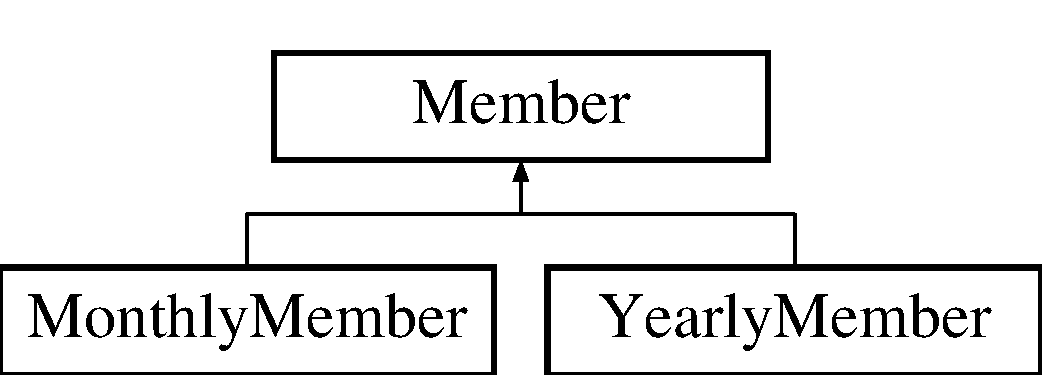
\includegraphics[height=2.000000cm]{class_member}
\end{center}
\end{figure}
\subsection*{Public Member Functions}
\begin{DoxyCompactItemize}
\item 
virtual \hyperlink{class_member}{Member} $\ast$ \hyperlink{class_member_a5011f255530d2994c6b99da470364fd7}{clone} ()=0
\item 
virtual void \hyperlink{class_member_ac8373d32ce216550cdc0302350130984}{pay\+Fee} (int num)=0
\item 
virtual void \hyperlink{class_member_ae854814cb8c9a456e84b6c284c47d230}{serialize} ()=0
\item 
{\footnotesize template$<$class Archive $>$ }\\void \hyperlink{class_member_a59f39205e0fa8712d1b5b245f74f0b82}{serialize} (Archive \&archive)
\end{DoxyCompactItemize}


\subsection{Member Function Documentation}
\index{Member@{Member}!clone@{clone}}
\index{clone@{clone}!Member@{Member}}
\subsubsection[{clone()=0}]{\setlength{\rightskip}{0pt plus 5cm}virtual {\bf Member}$\ast$ Member\+::clone (
\begin{DoxyParamCaption}
{}
\end{DoxyParamCaption}
)\hspace{0.3cm}{\ttfamily [pure virtual]}}\hypertarget{class_member_a5011f255530d2994c6b99da470364fd7}{}\label{class_member_a5011f255530d2994c6b99da470364fd7}


Implemented in \hyperlink{class_yearly_member_a6edc6f3be08787047c4a22c325046afa}{Yearly\+Member}, and \hyperlink{class_monthly_member_a24a5686d99977cc7ed9ed2c90b88cf0c}{Monthly\+Member}.

\index{Member@{Member}!pay\+Fee@{pay\+Fee}}
\index{pay\+Fee@{pay\+Fee}!Member@{Member}}
\subsubsection[{pay\+Fee(int num)=0}]{\setlength{\rightskip}{0pt plus 5cm}virtual void Member\+::pay\+Fee (
\begin{DoxyParamCaption}
\item[{int}]{num}
\end{DoxyParamCaption}
)\hspace{0.3cm}{\ttfamily [pure virtual]}}\hypertarget{class_member_ac8373d32ce216550cdc0302350130984}{}\label{class_member_ac8373d32ce216550cdc0302350130984}


Implemented in \hyperlink{class_yearly_member_a5beb8f8e9bb662dc963283c9bfa7773f}{Yearly\+Member}, and \hyperlink{class_monthly_member_ad5660394e1ed3126e7647f17c22e1875}{Monthly\+Member}.

\index{Member@{Member}!serialize@{serialize}}
\index{serialize@{serialize}!Member@{Member}}
\subsubsection[{serialize()=0}]{\setlength{\rightskip}{0pt plus 5cm}virtual void Member\+::serialize (
\begin{DoxyParamCaption}
{}
\end{DoxyParamCaption}
)\hspace{0.3cm}{\ttfamily [pure virtual]}}\hypertarget{class_member_ae854814cb8c9a456e84b6c284c47d230}{}\label{class_member_ae854814cb8c9a456e84b6c284c47d230}


Implemented in \hyperlink{class_yearly_member_af2b09fb2f659d449c32aee7107e3df03}{Yearly\+Member}, and \hyperlink{class_monthly_member_a2a0b8213862975e57a12b1bdabb7f8cb}{Monthly\+Member}.

\index{Member@{Member}!serialize@{serialize}}
\index{serialize@{serialize}!Member@{Member}}
\subsubsection[{serialize(\+Archive \&archive)}]{\setlength{\rightskip}{0pt plus 5cm}template$<$class Archive $>$ void Member\+::serialize (
\begin{DoxyParamCaption}
\item[{Archive \&}]{archive}
\end{DoxyParamCaption}
)\hspace{0.3cm}{\ttfamily [inline]}}\hypertarget{class_member_a59f39205e0fa8712d1b5b245f74f0b82}{}\label{class_member_a59f39205e0fa8712d1b5b245f74f0b82}


The documentation for this class was generated from the following file\+:\begin{DoxyCompactItemize}
\item 
assign2prototype/assign2prototype/\hyperlink{prototype_8cpp}{prototype.\+cpp}\end{DoxyCompactItemize}

\hypertarget{class_monthly_member}{}\section{Monthly\+Member Class Reference}
\label{class_monthly_member}\index{Monthly\+Member@{Monthly\+Member}}
Inheritance diagram for Monthly\+Member\+:\begin{figure}[H]
\begin{center}
\leavevmode
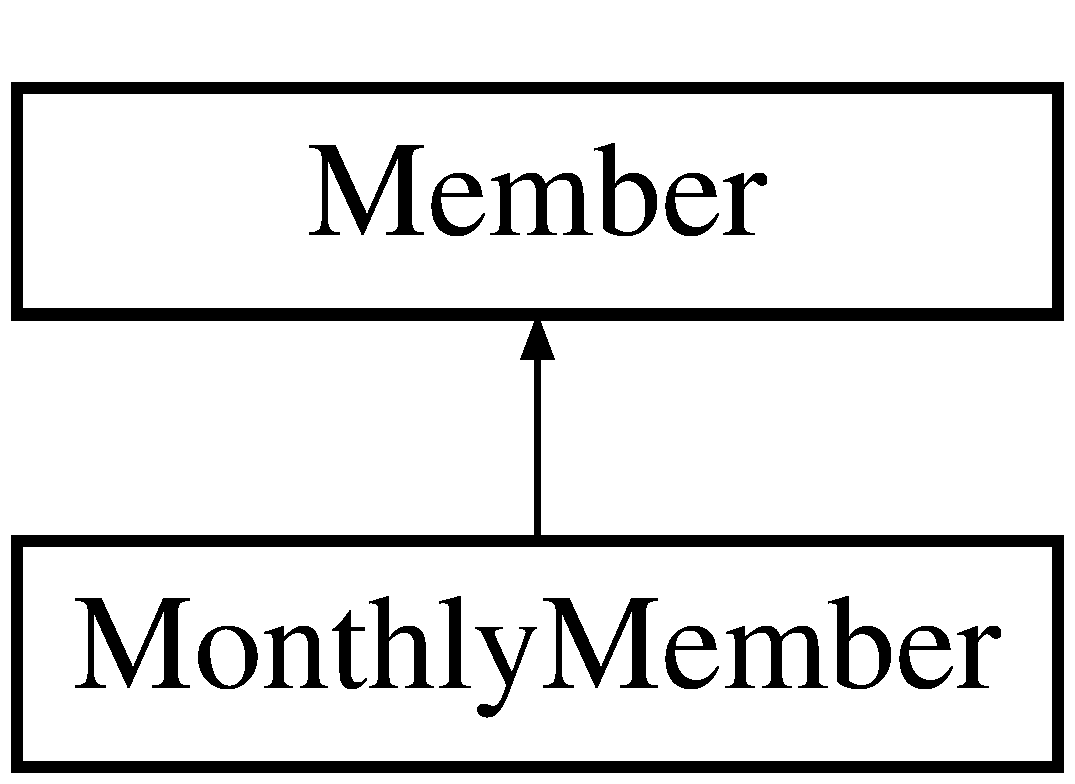
\includegraphics[height=2.000000cm]{class_monthly_member}
\end{center}
\end{figure}
\subsection*{Public Member Functions}
\begin{DoxyCompactItemize}
\item 
\hyperlink{class_member}{Member} $\ast$ \hyperlink{class_monthly_member_a24a5686d99977cc7ed9ed2c90b88cf0c}{clone} ()
\item 
void \hyperlink{class_monthly_member_ad5660394e1ed3126e7647f17c22e1875}{pay\+Fee} (int num)
\item 
void \hyperlink{class_monthly_member_a2a0b8213862975e57a12b1bdabb7f8cb}{serialize} ()
\end{DoxyCompactItemize}


\subsection{Member Function Documentation}
\index{Monthly\+Member@{Monthly\+Member}!clone@{clone}}
\index{clone@{clone}!Monthly\+Member@{Monthly\+Member}}
\subsubsection[{clone()}]{\setlength{\rightskip}{0pt plus 5cm}{\bf Member}$\ast$ Monthly\+Member\+::clone (
\begin{DoxyParamCaption}
{}
\end{DoxyParamCaption}
)\hspace{0.3cm}{\ttfamily [inline]}, {\ttfamily [virtual]}}\hypertarget{class_monthly_member_a24a5686d99977cc7ed9ed2c90b88cf0c}{}\label{class_monthly_member_a24a5686d99977cc7ed9ed2c90b88cf0c}


Implements \hyperlink{class_member_a5011f255530d2994c6b99da470364fd7}{Member}.

\index{Monthly\+Member@{Monthly\+Member}!pay\+Fee@{pay\+Fee}}
\index{pay\+Fee@{pay\+Fee}!Monthly\+Member@{Monthly\+Member}}
\subsubsection[{pay\+Fee(int num)}]{\setlength{\rightskip}{0pt plus 5cm}void Monthly\+Member\+::pay\+Fee (
\begin{DoxyParamCaption}
\item[{int}]{num}
\end{DoxyParamCaption}
)\hspace{0.3cm}{\ttfamily [inline]}, {\ttfamily [virtual]}}\hypertarget{class_monthly_member_ad5660394e1ed3126e7647f17c22e1875}{}\label{class_monthly_member_ad5660394e1ed3126e7647f17c22e1875}


Implements \hyperlink{class_member_ac8373d32ce216550cdc0302350130984}{Member}.

\index{Monthly\+Member@{Monthly\+Member}!serialize@{serialize}}
\index{serialize@{serialize}!Monthly\+Member@{Monthly\+Member}}
\subsubsection[{serialize()}]{\setlength{\rightskip}{0pt plus 5cm}void Monthly\+Member\+::serialize (
\begin{DoxyParamCaption}
{}
\end{DoxyParamCaption}
)\hspace{0.3cm}{\ttfamily [inline]}, {\ttfamily [virtual]}}\hypertarget{class_monthly_member_a2a0b8213862975e57a12b1bdabb7f8cb}{}\label{class_monthly_member_a2a0b8213862975e57a12b1bdabb7f8cb}


Implements \hyperlink{class_member_ae854814cb8c9a456e84b6c284c47d230}{Member}.



The documentation for this class was generated from the following file\+:\begin{DoxyCompactItemize}
\item 
assign2prototype/assign2prototype/\hyperlink{prototype_8cpp}{prototype.\+cpp}\end{DoxyCompactItemize}

\hypertarget{class_ptr}{}\section{Ptr Class Reference}
\label{class_ptr}\index{Ptr@{Ptr}}
\subsection*{Public Member Functions}
\begin{DoxyCompactItemize}
\item 
\hyperlink{class_ptr_a3a3ae84b911eb202b69f5cf6b56c5190}{Ptr} (\hyperlink{class_member}{Member} $\ast$p=N\+U\+LL)
\item 
\hyperlink{class_ptr_a91279a893ef126e4e8584f60c2a0f0da}{$\sim$\+Ptr} ()
\item 
\hyperlink{class_member}{Member} \& \hyperlink{class_ptr_a8bd7cd908143eec22d9c3029471c6206}{operator$\ast$} ()
\item 
{\footnotesize template$<$class Archive $>$ }\\void \hyperlink{class_ptr_acd6e4735e8593314678639432f1f4b7b}{serialize} (Archive \&archive)
\end{DoxyCompactItemize}


\subsection{Constructor \& Destructor Documentation}
\index{Ptr@{Ptr}!Ptr@{Ptr}}
\index{Ptr@{Ptr}!Ptr@{Ptr}}
\subsubsection[{Ptr(\+Member $\ast$p=\+N\+U\+L\+L)}]{\setlength{\rightskip}{0pt plus 5cm}Ptr\+::\+Ptr (
\begin{DoxyParamCaption}
\item[{{\bf Member} $\ast$}]{p = {\ttfamily NULL}}
\end{DoxyParamCaption}
)\hspace{0.3cm}{\ttfamily [inline]}, {\ttfamily [explicit]}}\hypertarget{class_ptr_a3a3ae84b911eb202b69f5cf6b56c5190}{}\label{class_ptr_a3a3ae84b911eb202b69f5cf6b56c5190}
\index{Ptr@{Ptr}!````~Ptr@{$\sim$\+Ptr}}
\index{````~Ptr@{$\sim$\+Ptr}!Ptr@{Ptr}}
\subsubsection[{$\sim$\+Ptr()}]{\setlength{\rightskip}{0pt plus 5cm}Ptr\+::$\sim$\+Ptr (
\begin{DoxyParamCaption}
{}
\end{DoxyParamCaption}
)\hspace{0.3cm}{\ttfamily [inline]}}\hypertarget{class_ptr_a91279a893ef126e4e8584f60c2a0f0da}{}\label{class_ptr_a91279a893ef126e4e8584f60c2a0f0da}


\subsection{Member Function Documentation}
\index{Ptr@{Ptr}!operator$\ast$@{operator$\ast$}}
\index{operator$\ast$@{operator$\ast$}!Ptr@{Ptr}}
\subsubsection[{operator$\ast$()}]{\setlength{\rightskip}{0pt plus 5cm}{\bf Member}\& Ptr\+::operator$\ast$ (
\begin{DoxyParamCaption}
{}
\end{DoxyParamCaption}
)\hspace{0.3cm}{\ttfamily [inline]}}\hypertarget{class_ptr_a8bd7cd908143eec22d9c3029471c6206}{}\label{class_ptr_a8bd7cd908143eec22d9c3029471c6206}
\index{Ptr@{Ptr}!serialize@{serialize}}
\index{serialize@{serialize}!Ptr@{Ptr}}
\subsubsection[{serialize(\+Archive \&archive)}]{\setlength{\rightskip}{0pt plus 5cm}template$<$class Archive $>$ void Ptr\+::serialize (
\begin{DoxyParamCaption}
\item[{Archive \&}]{archive}
\end{DoxyParamCaption}
)\hspace{0.3cm}{\ttfamily [inline]}}\hypertarget{class_ptr_acd6e4735e8593314678639432f1f4b7b}{}\label{class_ptr_acd6e4735e8593314678639432f1f4b7b}


The documentation for this class was generated from the following file\+:\begin{DoxyCompactItemize}
\item 
assign2prototype/assign2prototype/\hyperlink{prototype_8cpp}{prototype.\+cpp}\end{DoxyCompactItemize}

\hypertarget{class_yearly_member}{}\section{Yearly\+Member Class Reference}
\label{class_yearly_member}\index{Yearly\+Member@{Yearly\+Member}}
Inheritance diagram for Yearly\+Member\+:\begin{figure}[H]
\begin{center}
\leavevmode
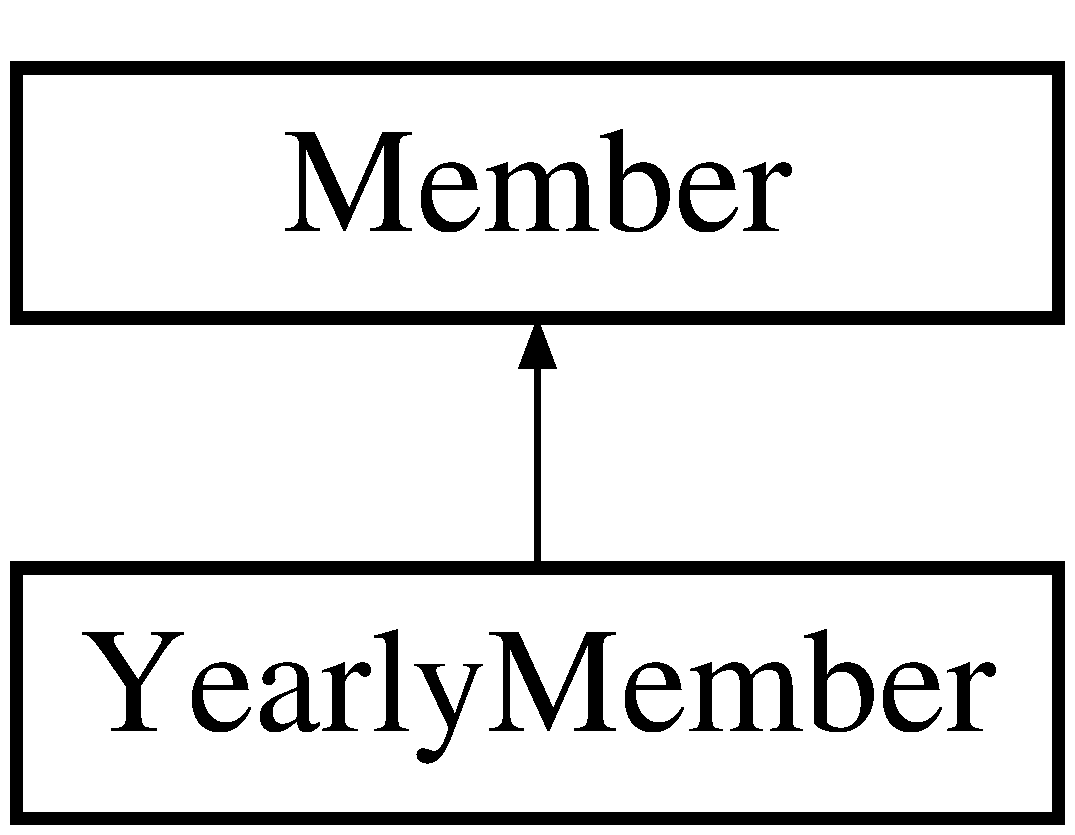
\includegraphics[height=2.000000cm]{class_yearly_member}
\end{center}
\end{figure}
\subsection*{Public Member Functions}
\begin{DoxyCompactItemize}
\item 
\hyperlink{class_member}{Member} $\ast$ \hyperlink{class_yearly_member_a6edc6f3be08787047c4a22c325046afa}{clone} ()
\item 
void \hyperlink{class_yearly_member_a5beb8f8e9bb662dc963283c9bfa7773f}{pay\+Fee} (int num)
\item 
void \hyperlink{class_yearly_member_af2b09fb2f659d449c32aee7107e3df03}{serialize} ()
\end{DoxyCompactItemize}


\subsection{Member Function Documentation}
\index{Yearly\+Member@{Yearly\+Member}!clone@{clone}}
\index{clone@{clone}!Yearly\+Member@{Yearly\+Member}}
\subsubsection[{clone()}]{\setlength{\rightskip}{0pt plus 5cm}{\bf Member}$\ast$ Yearly\+Member\+::clone (
\begin{DoxyParamCaption}
{}
\end{DoxyParamCaption}
)\hspace{0.3cm}{\ttfamily [inline]}, {\ttfamily [virtual]}}\hypertarget{class_yearly_member_a6edc6f3be08787047c4a22c325046afa}{}\label{class_yearly_member_a6edc6f3be08787047c4a22c325046afa}


Implements \hyperlink{class_member_a5011f255530d2994c6b99da470364fd7}{Member}.

\index{Yearly\+Member@{Yearly\+Member}!pay\+Fee@{pay\+Fee}}
\index{pay\+Fee@{pay\+Fee}!Yearly\+Member@{Yearly\+Member}}
\subsubsection[{pay\+Fee(int num)}]{\setlength{\rightskip}{0pt plus 5cm}void Yearly\+Member\+::pay\+Fee (
\begin{DoxyParamCaption}
\item[{int}]{num}
\end{DoxyParamCaption}
)\hspace{0.3cm}{\ttfamily [inline]}, {\ttfamily [virtual]}}\hypertarget{class_yearly_member_a5beb8f8e9bb662dc963283c9bfa7773f}{}\label{class_yearly_member_a5beb8f8e9bb662dc963283c9bfa7773f}


Implements \hyperlink{class_member_ac8373d32ce216550cdc0302350130984}{Member}.

\index{Yearly\+Member@{Yearly\+Member}!serialize@{serialize}}
\index{serialize@{serialize}!Yearly\+Member@{Yearly\+Member}}
\subsubsection[{serialize()}]{\setlength{\rightskip}{0pt plus 5cm}void Yearly\+Member\+::serialize (
\begin{DoxyParamCaption}
{}
\end{DoxyParamCaption}
)\hspace{0.3cm}{\ttfamily [inline]}, {\ttfamily [virtual]}}\hypertarget{class_yearly_member_af2b09fb2f659d449c32aee7107e3df03}{}\label{class_yearly_member_af2b09fb2f659d449c32aee7107e3df03}


Implements \hyperlink{class_member_ae854814cb8c9a456e84b6c284c47d230}{Member}.



The documentation for this class was generated from the following file\+:\begin{DoxyCompactItemize}
\item 
assign2prototype/assign2prototype/\hyperlink{prototype_8cpp}{prototype.\+cpp}\end{DoxyCompactItemize}

\chapter{File Documentation}
\hypertarget{prototype_8cpp}{}\section{assign2prototype/assign2prototype/prototype.cpp File Reference}
\label{prototype_8cpp}\index{assign2prototype/assign2prototype/prototype.\+cpp@{assign2prototype/assign2prototype/prototype.\+cpp}}
{\ttfamily \#include $<$iostream$>$}\\*
{\ttfamily \#include $<$string$>$}\\*
{\ttfamily \#include $<$vector$>$}\\*
{\ttfamily \#include $<$fstream$>$}\\*
{\ttfamily \#include $<$cereal/archives/json.\+hpp$>$}\\*
{\ttfamily \#include $<$cereal/types/vector.\+hpp$>$}\\*
{\ttfamily \#include $<$cereal/types/memory.\+hpp$>$}\\*
\subsection*{Classes}
\begin{DoxyCompactItemize}
\item 
class \hyperlink{class_member}{Member}
\item 
class \hyperlink{class_factory}{Factory}
\item 
class \hyperlink{class_monthly_member}{Monthly\+Member}
\item 
class \hyperlink{class_yearly_member}{Yearly\+Member}
\item 
class \hyperlink{class_ptr}{Ptr}
\end{DoxyCompactItemize}
\subsection*{Functions}
\begin{DoxyCompactItemize}
\item 
int \hyperlink{prototype_8cpp_ae66f6b31b5ad750f1fe042a706a4e3d4}{main} ()
\end{DoxyCompactItemize}


\subsection{Function Documentation}
\index{prototype.\+cpp@{prototype.\+cpp}!main@{main}}
\index{main@{main}!prototype.\+cpp@{prototype.\+cpp}}
\subsubsection[{main()}]{\setlength{\rightskip}{0pt plus 5cm}int main (
\begin{DoxyParamCaption}
{}
\end{DoxyParamCaption}
)}\hypertarget{prototype_8cpp_ae66f6b31b5ad750f1fe042a706a4e3d4}{}\label{prototype_8cpp_ae66f6b31b5ad750f1fe042a706a4e3d4}

%--- End generated contents ---

% Index
\backmatter
\newpage
\phantomsection
\clearemptydoublepage
\addcontentsline{toc}{chapter}{Index}
\printindex

\end{document}
